\setcounter{definition}{0} \setcounter{property}{0} \setcounter{claim}{0} \setcounter{fact}{0} \setcounter{corollary}{0} \setcounter{figure}{0}
\setcounter{definition}{0} \setcounter{property}{0} \setcounter{claim}{0} \setcounter{fact}{0} \setcounter{corollary}{0}
\section{The 2SAT Problem}

\subsection*{Boolean Satisfiability Problem}

The SAT problem~(Boolean Satisfiability Problem) is 
to decide if a given boolean formula can be satisfied
by assigning values to boolean variables.
Let's define it. The \emph{variables}, $x_1, x_2, \cdots, x_m$, involved are
boolean~(or binary), taking value of either true or false.
A \emph{literal} is either a variable itself~(e.g., $x_3$, $x_5$, etc) or the negation of a variable~(e.g., $\overline{x_3}$, $\overline{x_5}$, etc).
A \emph{clause} is a disjunction of literals~(e.g., $x_2 \vee \overline{x_4}$, $\overline{x_3} \vee \overline{x_5} \vee x_2$, $\overline{x_1}$, etc).
A \emph{CNF~(conjunctive normal form) formula} is a conjunction of clauses, such as  
$(x_2 \vee \overline{x_4})\wedge (\overline{x_3} \vee \overline{x_5} \vee x_2) \wedge (\overline{x_1})$.

Given a CNF formula with $n$ clauses $C_1, C_2, \cdots, C_n$ involving $m$ variables
$x_1, x_2, \cdots, x_m$, the SAT problem is to decide if there exists an
\emph{assignment}~(i.e., assigning true or false value to each variable) such
that all $n$ clauses are true~(i.e., the CNF formula is true).

If each clause is restricted to have exactly 3 literals, then the above problem becomes the so-called 3SAT problem.
3SAT has been proved to be NP-hard, i.e., there doesn't exist any efficient algorithm for it unless P~=~NP.
(We will introduce NP-completeness later this course; you don't need to know that these mean now.)

If each clause is restricted to have exactly 2 literals, then the above problem becomes the 2SAT problem.
2SAT can be solved efficiently, actually in $\Theta(m + n)$ time.
Below we will design an algorithm for 2SAT, in which the core part is to use the algorithm of identifying connected componenets of directed graphs.

\subsection*{Implication Graph and Algorithm}

A clause with 2 literals represents two implication relationship.
For example, consider clause $\overline{x_1} \vee x_2$.
In order to satisfy it, if $\overline{x_1}$ is false then $x_2$ must be true, and  
if $x_2$ is false then $\overline{x_1}$ must be true.  
Formally, we have

\begin{fact}
Clause $A\vee B$ is equivalent to $\overline{A} \Rightarrow B$ and $\overline{B} \Rightarrow A$.
Here $A$ or $B$ represents any literal~(i.e., either a variable or the negation of a variable),
and $\Rightarrow$ represents logic ``implication''.
\end{fact}

\begin{figure}[b!]
\centering{

\tikzset{every picture/.style={line width=0.75pt}} %set default line width to 0.75pt        

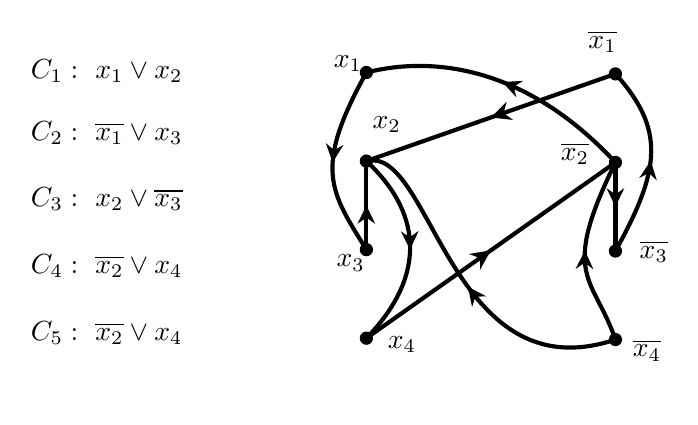
\begin{tikzpicture}[x=0.5pt,y=0.5pt,yscale=-1,xscale=1]
%uncomment if require: \path (0,248); %set diagram left start at 0, and has height of 248

%Flowchart: Connector [id:dp5285899162991353] 
\draw  [fill={rgb, 255:red, 0; green, 0; blue, 0 }  ,fill opacity=1 ] (252,32) .. controls (252,29.58) and (253.96,27.62) .. (256.38,27.62) .. controls (258.79,27.62) and (260.75,29.58) .. (260.75,32) .. controls (260.75,34.42) and (258.79,36.38) .. (256.38,36.38) .. controls (253.96,36.38) and (252,34.42) .. (252,32) -- cycle ;
%Straight Lines [id:da03484807968209058] 
\draw [color={rgb, 255:red, 0; green, 0; blue, 0 }  ,draw opacity=1 ][line width=1.5]    (256.38,224) -- (436.38,97) ;
\draw [shift={(346.38,160.5)}, rotate = 504.8] [fill={rgb, 255:red, 0; green, 0; blue, 0 }  ,fill opacity=1 ][line width=0.08]  [draw opacity=0] (14.56,-6.99) -- (0,0) -- (14.56,6.99) -- (9.67,0) -- cycle    ;
%Flowchart: Connector [id:dp28963957089609804] 
\draw  [fill={rgb, 255:red, 0; green, 0; blue, 0 }  ,fill opacity=1 ] (252,96) .. controls (252,93.59) and (253.96,91.63) .. (256.38,91.63) .. controls (258.79,91.63) and (260.75,93.59) .. (260.75,96) .. controls (260.75,98.42) and (258.79,100.38) .. (256.38,100.38) .. controls (253.96,100.38) and (252,98.42) .. (252,96) -- cycle ;
%Flowchart: Connector [id:dp5510231189769008] 
\draw  [fill={rgb, 255:red, 0; green, 0; blue, 0 }  ,fill opacity=1 ] (252,160.01) .. controls (252,157.59) and (253.96,155.63) .. (256.38,155.63) .. controls (258.79,155.63) and (260.75,157.59) .. (260.75,160.01) .. controls (260.75,162.42) and (258.79,164.38) .. (256.38,164.38) .. controls (253.96,164.38) and (252,162.42) .. (252,160.01) -- cycle ;
%Flowchart: Connector [id:dp8347416280872515] 
\draw  [fill={rgb, 255:red, 0; green, 0; blue, 0 }  ,fill opacity=1 ] (252,224) .. controls (252,221.58) and (253.96,219.62) .. (256.38,219.62) .. controls (258.79,219.62) and (260.75,221.58) .. (260.75,224) .. controls (260.75,226.42) and (258.79,228.38) .. (256.38,228.38) .. controls (253.96,228.38) and (252,226.42) .. (252,224) -- cycle ;
%Flowchart: Connector [id:dp09589448620018437] 
\draw  [fill={rgb, 255:red, 0; green, 0; blue, 0 }  ,fill opacity=1 ] (432,33) .. controls (432,30.58) and (433.96,28.62) .. (436.38,28.62) .. controls (438.79,28.62) and (440.75,30.58) .. (440.75,33) .. controls (440.75,35.42) and (438.79,37.38) .. (436.38,37.38) .. controls (433.96,37.38) and (432,35.42) .. (432,33) -- cycle ;
%Flowchart: Connector [id:dp6276853107817513] 
\draw  [fill={rgb, 255:red, 0; green, 0; blue, 0 }  ,fill opacity=1 ] (432,97) .. controls (432,94.59) and (433.96,92.63) .. (436.38,92.63) .. controls (438.79,92.63) and (440.75,94.59) .. (440.75,97) .. controls (440.75,99.42) and (438.79,101.38) .. (436.38,101.38) .. controls (433.96,101.38) and (432,99.42) .. (432,97) -- cycle ;
%Flowchart: Connector [id:dp7176343531829045] 
\draw  [fill={rgb, 255:red, 0; green, 0; blue, 0 }  ,fill opacity=1 ] (432,161.01) .. controls (432,158.59) and (433.96,156.63) .. (436.38,156.63) .. controls (438.79,156.63) and (440.75,158.59) .. (440.75,161.01) .. controls (440.75,163.42) and (438.79,165.38) .. (436.38,165.38) .. controls (433.96,165.38) and (432,163.42) .. (432,161.01) -- cycle ;
%Flowchart: Connector [id:dp8859571266882346] 
\draw  [fill={rgb, 255:red, 0; green, 0; blue, 0 }  ,fill opacity=1 ] (432,225) .. controls (432,222.58) and (433.96,220.62) .. (436.38,220.62) .. controls (438.79,220.62) and (440.75,222.58) .. (440.75,225) .. controls (440.75,227.42) and (438.79,229.38) .. (436.38,229.38) .. controls (433.96,229.38) and (432,227.42) .. (432,225) -- cycle ;
%Straight Lines [id:da9353211071842927] 
\draw [color={rgb, 255:red, 0; green, 0; blue, 0 }  ,draw opacity=1 ][line width=1.5]    (436.38,33) -- (256.38,96) ;
\draw [shift={(346.38,64.5)}, rotate = 340.71000000000004] [fill={rgb, 255:red, 0; green, 0; blue, 0 }  ,fill opacity=1 ][line width=0.08]  [draw opacity=0] (14.56,-6.99) -- (0,0) -- (14.56,6.99) -- (9.67,0) -- cycle    ;
%Straight Lines [id:da07119264102777723] 
\draw [line width=1.5]    (256.38,160.01) -- (256.38,96) ;
\draw [shift={(256.38,128)}, rotate = 450] [fill={rgb, 255:red, 0; green, 0; blue, 0 }  ][line width=0.08]  [draw opacity=0] (13.4,-6.43) -- (0,0) -- (13.4,6.44) -- (8.9,0) -- cycle    ;
%Curve Lines [id:da7435687764576437] 
\draw [line width=1.5]    (436.38,97) .. controls (371.5,27) and (303.5,20) .. (256.38,32) ;
\draw [shift={(354.76,38.88)}, rotate = 382.41999999999996] [fill={rgb, 255:red, 0; green, 0; blue, 0 }  ][line width=0.08]  [draw opacity=0] (13.4,-6.43) -- (0,0) -- (13.4,6.44) -- (8.9,0) -- cycle    ;
%Curve Lines [id:da5802575901273257] 
\draw [line width=1.5]    (256.38,96) .. controls (300.5,137) and (296.5,183) .. (256.38,224) ;
\draw [shift={(287.97,160)}, rotate = 268.81] [fill={rgb, 255:red, 0; green, 0; blue, 0 }  ][line width=0.08]  [draw opacity=0] (13.4,-6.43) -- (0,0) -- (13.4,6.44) -- (8.9,0) -- cycle    ;
%Curve Lines [id:da7175218471577676] 
\draw [line width=1.5]    (436.38,225) .. controls (420.5,179) and (395.5,180) .. (436.38,97) ;
\draw [shift={(414.3,160.68)}, rotate = 451.13] [fill={rgb, 255:red, 0; green, 0; blue, 0 }  ][line width=0.08]  [draw opacity=0] (13.4,-6.43) -- (0,0) -- (13.4,6.44) -- (8.9,0) -- cycle    ;
%Curve Lines [id:da6924159573089901] 
\draw [line width=1.5]    (256.38,32) .. controls (217.5,102) and (230.5,118) .. (256.38,160.01) ;
\draw [shift={(231.99,96.97)}, rotate = 276.2] [fill={rgb, 255:red, 0; green, 0; blue, 0 }  ][line width=0.08]  [draw opacity=0] (13.4,-6.43) -- (0,0) -- (13.4,6.44) -- (8.9,0) -- cycle    ;
%Curve Lines [id:da35461450717449705] 
\draw [line width=1.5]    (436.38,161.01) .. controls (469.12,102) and (472.5,73) .. (436.38,33) ;
\draw [shift={(461.82,95.84)}, rotate = 458.06] [fill={rgb, 255:red, 0; green, 0; blue, 0 }  ][line width=0.08]  [draw opacity=0] (13.4,-6.43) -- (0,0) -- (13.4,6.44) -- (8.9,0) -- cycle    ;
%Straight Lines [id:da1097593932252855] 
\draw [line width=1.5]    (436.38,97) -- (436.38,161.01) ;
\draw [shift={(436.38,129)}, rotate = 270] [fill={rgb, 255:red, 0; green, 0; blue, 0 }  ][line width=0.08]  [draw opacity=0] (13.4,-6.43) -- (0,0) -- (13.4,6.44) -- (8.9,0) -- cycle    ;
%Curve Lines [id:da37464522628067776] 
\draw [line width=1.5]    (436.38,225) .. controls (316.5,265) and (303.5,84) .. (256.38,96) ;
\draw [shift={(329.81,186.93)}, rotate = 412.86] [fill={rgb, 255:red, 0; green, 0; blue, 0 }  ][line width=0.08]  [draw opacity=0] (13.4,-6.43) -- (0,0) -- (13.4,6.44) -- (8.9,0) -- cycle    ;

% Text Node
\draw (12,21) node [anchor=north west][inner sep=0.75pt]   [align=left] {$\displaystyle C_{1} :\ x_{1} \lor x_{2}$};
% Text Node
\draw (12,65.25) node [anchor=north west][inner sep=0.75pt]   [align=left] {$\displaystyle C_{2} :\ \overline{x_{1}} \lor x_{3}$};
% Text Node
\draw (12,113.5) node [anchor=north west][inner sep=0.75pt]   [align=left] {$\displaystyle C_{3} :\ x_{2} \lor \overline{x_{3}}$};
% Text Node
\draw (12,161.75) node [anchor=north west][inner sep=0.75pt]   [align=left] {$\displaystyle C_{4} :\ \overline{x_{2}} \lor x_{4}$};
% Text Node
\draw (12,210) node [anchor=north west][inner sep=0.75pt]   [align=left] {$\displaystyle C_{5} :\ \overline{x_{2}} \lor x_{4}$};
% Text Node
\draw (231,18) node [anchor=north west][inner sep=0.75pt]   [align=left] {$\displaystyle x_{1}$};
% Text Node
\draw (259,62) node [anchor=north west][inner sep=0.75pt]   [align=left] {$\displaystyle x_{2}$};
% Text Node
\draw (233,162) node [anchor=north west][inner sep=0.75pt]   [align=left] {$\displaystyle x_{3}$};
% Text Node
\draw (270,221) node [anchor=north west][inner sep=0.75pt]   [align=left] {$\displaystyle x_{4}$};
% Text Node
\draw (415,0) node [anchor=north west][inner sep=0.75pt]   [align=left] {$\displaystyle \overline{x_{1}}$};
% Text Node
\draw (395,81) node [anchor=north west][inner sep=0.75pt]   [align=left] {$\displaystyle \overline{x_{2}}$};
% Text Node
\draw (452,152) node [anchor=north west][inner sep=0.75pt]   [align=left] {$\displaystyle \overline{x_{3}}$};
% Text Node
\draw (447,223) node [anchor=north west][inner sep=0.75pt]   [align=left] {$\displaystyle \overline{x_{4}}$};


\end{tikzpicture}

}
\caption{Graph and its reverse graph, and the corresponding meta-graphs.}
\label{fig:instance1}
\end{figure}

We can then use a directed graph $G = (V,E)$, called implication graph, to represent all such implications of the given $n$ clauses~(with $m$ variables).
The graph contains $2m$ vertices, corresponding to all possible literals, i.e.,
$V = \{x_1, \overline{x_1}, x_2, \overline{x_2}, \cdots, x_n, \overline{x_n}\}$.
And the graph contains $2n$ edges: each clause $A\vee B$ corresponds to 2 edges in $G$, which are $(\overline{A}, B)$ and $(\overline{B}, A)$.
Intuitively, an edge $(u,v)\in E$ represents, if literal $u$ is true then literal $v$ must be true.
An example of implication graph is given in Figure~\ref{fig:instance1}.

%\begin{fact}
%In an implication graph $G = (V,E)$ there exists an edge $(u,v)$ if and only if there exists edge $(\overline{v}, \overline{u})$.
%\end{fact}

The implication can be carrying forward following any path in the implication graph. For example, path
$u\to v \to w$ implies that if literal $u$ is true then literal $w$ must be
true. What if there is path from $u$ to $\overline{u}$?
This means that: if literal $u$ is true then $\overline{u}$ must be true, which is a contradiction.
Hence, if such path exists then literal $u$ can't be true.
What if there is path from $u$ to $\overline{u}$ \emph{and}
there is path from $\overline{u}$ to $v$?
Then this means that $u$ can't be true \emph{and} $\overline{u}$ can't be true.
In other words, the instance is not satisfiable.
We summarize as the following statement. 

\begin{fact}
If in the implication graph there is a path from literal $u$ to literal $\overline{u}$ and there is a
path from literal $\overline{u}$ to literal $u$, then the instance is not satisfiable.
\end{fact}

The above fact gives a sufficient condition to decide if an 2SAT instance is not satisfiable.
In fact, this condition is also necessary. We will prove it later on.
Before that, let's design an algorithm to implement this condition, i.e., to decide if there
exists a pair of literals $\{u,\overline{u}\}$ such that $u$ can reach $\overline{u}$ and $\overline{u}$ can reach $u$.

A straightforward algorithm is to explore~($G$, $u$) and explore~($G$, $\overline{u}$), for every pair of literals.
This takes $O(|V|\cdot |E|)$ time, as a single run of explore takes $O(|E|)$ time. Can we do better?

Note that the condition that $u$ can reach $\overline{u}$ and $\overline{u}$ can reach $u$
is equivalent to that $u$ and $\overline{u}$ are in the same connected component of $G$.
Therefore, we can use the algorithm introduced in previous lecture to determine all connected components of $G$, which takes $\Theta(|V| + |E|)$ time.
Then we can simply check the resulting $visited$ array: if a pair of literals satisfies $visited[u] = visited[\overline{u}]$ then the 2SAT instance is not satisfiable.
The pseudo-code is given below.

\begin{minipage}{0.8\textwidth}
	\aaA {7}{Algorithm decide-2SAT ($C_1, C_2, \cdots, C_n$)}\xxx
	\aab {build implication graph $G = (V, E)$;}\xxx
	\aab {run the DFS algorithm to find all connected components of $G$; this gives $visited$ array;}\xxx
	\aaB {2}{for each pair of literals $\{u, \overline{u}\}$}\xxx
	\aac {if ($visited[u] = visited[\overline{u}]$): return false;}\xxx
	\aab {end for;}\xxx
	\aab {return true;}\xxx
	\aaa {end algorithm;}\xxx
\end{minipage}

We showed that if there exists $u$ and $\overline{u}$ that are in the same connected
component, then the 2SAT instance is not satisfiable, i.e., the above
algorithm is correct when returning false.  We now show that if such
pair does not exists, then the 2SAT instance is satisfiable, i.e., the
above algorithm is correct when returning true.
The proof is constructive, i.e., when such pair does not exist, we can
build an assignment that satisfies all clauses.
The algorithm to find such an assignment is as follows. %~(see Figure~\ref{fig:instance2}).
%We find a linearization $X$ of the meta-graph of $G$. (Think: how?)

\begin{minipage}{0.8\textwidth}
	\aaA {8}{Algorithm build-assignment~($C_1, C_2, \cdots, C_n$)}\xxx
	\aab {run above decide-2SAT algorithm and assume it returns true;}\xxx
	\aab {build a linearization $X$ of the meta-graph $G^M$ of the implication graph $G$;}\xxx
	\aaB {4}{for each pair of literals $\{u, \overline{u}\}$}\xxx
	\aac {let $C(u) = visited[u]$ and  $C(\overline{u}) = visited[\overline{u}]$ be the components that include $u$ and $\overline{u}$, respectively;}\xxx
	\aac {if $C(u)$ is before $C(\overline{u})$ in $X$: set literal $u$ to false and $\overline{u}$ to true;}\xxx
	\aac {if $C(u)$ is after $C(\overline{u})$ in $X$: set literal $u$ to true and $\overline{u}$ to false;}\xxx
	\aab {end for;}\xxx
	\aaa {end algorithm;}\xxx
\end{minipage}

%Before proving that above algorithm gives an assignment that satisfies all clauses,
Try to run above algorithm on the example given in Figure~\ref{fig:instance2}.

\begin{figure}[h!]
\centering{

\tikzset{every picture/.style={line width=0.75pt}} %set default line width to 0.75pt        

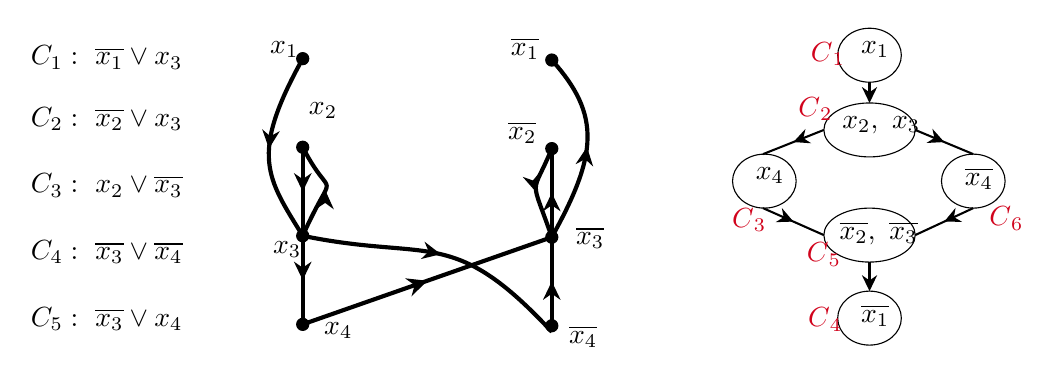
\begin{tikzpicture}[x=0.5pt,y=0.5pt,yscale=-1,xscale=1]
%uncomment if require: \path (0,257); %set diagram left start at 0, and has height of 257

%Flowchart: Connector [id:dp3724199168464428] 
\draw  [fill={rgb, 255:red, 0; green, 0; blue, 0 }  ,fill opacity=1 ] (206,32) .. controls (206,29.58) and (207.96,27.62) .. (210.38,27.62) .. controls (212.79,27.62) and (214.75,29.58) .. (214.75,32) .. controls (214.75,34.42) and (212.79,36.38) .. (210.38,36.38) .. controls (207.96,36.38) and (206,34.42) .. (206,32) -- cycle ;
%Straight Lines [id:da21698138157344438] 
\draw [color={rgb, 255:red, 0; green, 0; blue, 0 }  ,draw opacity=1 ][line width=1.5]    (210.38,224) -- (390.38,161.01) ;
\draw [shift={(300.38,192.5)}, rotate = 520.71] [fill={rgb, 255:red, 0; green, 0; blue, 0 }  ,fill opacity=1 ][line width=0.08]  [draw opacity=0] (14.56,-6.99) -- (0,0) -- (14.56,6.99) -- (9.67,0) -- cycle    ;
%Flowchart: Connector [id:dp10381668129107124] 
\draw  [fill={rgb, 255:red, 0; green, 0; blue, 0 }  ,fill opacity=1 ] (206,96) .. controls (206,93.59) and (207.96,91.63) .. (210.38,91.63) .. controls (212.79,91.63) and (214.75,93.59) .. (214.75,96) .. controls (214.75,98.42) and (212.79,100.38) .. (210.38,100.38) .. controls (207.96,100.38) and (206,98.42) .. (206,96) -- cycle ;
%Flowchart: Connector [id:dp3907425587900879] 
\draw  [fill={rgb, 255:red, 0; green, 0; blue, 0 }  ,fill opacity=1 ] (206,160.01) .. controls (206,157.59) and (207.96,155.63) .. (210.38,155.63) .. controls (212.79,155.63) and (214.75,157.59) .. (214.75,160.01) .. controls (214.75,162.42) and (212.79,164.38) .. (210.38,164.38) .. controls (207.96,164.38) and (206,162.42) .. (206,160.01) -- cycle ;
%Flowchart: Connector [id:dp7417499401424387] 
\draw  [fill={rgb, 255:red, 0; green, 0; blue, 0 }  ,fill opacity=1 ] (206,224) .. controls (206,221.58) and (207.96,219.62) .. (210.38,219.62) .. controls (212.79,219.62) and (214.75,221.58) .. (214.75,224) .. controls (214.75,226.42) and (212.79,228.38) .. (210.38,228.38) .. controls (207.96,228.38) and (206,226.42) .. (206,224) -- cycle ;
%Flowchart: Connector [id:dp6925277380251512] 
\draw  [fill={rgb, 255:red, 0; green, 0; blue, 0 }  ,fill opacity=1 ] (386,33) .. controls (386,30.58) and (387.96,28.62) .. (390.38,28.62) .. controls (392.79,28.62) and (394.75,30.58) .. (394.75,33) .. controls (394.75,35.42) and (392.79,37.38) .. (390.38,37.38) .. controls (387.96,37.38) and (386,35.42) .. (386,33) -- cycle ;
%Flowchart: Connector [id:dp39532236220272543] 
\draw  [fill={rgb, 255:red, 0; green, 0; blue, 0 }  ,fill opacity=1 ] (386,97) .. controls (386,94.59) and (387.96,92.63) .. (390.38,92.63) .. controls (392.79,92.63) and (394.75,94.59) .. (394.75,97) .. controls (394.75,99.42) and (392.79,101.38) .. (390.38,101.38) .. controls (387.96,101.38) and (386,99.42) .. (386,97) -- cycle ;
%Flowchart: Connector [id:dp9098235514745779] 
\draw  [fill={rgb, 255:red, 0; green, 0; blue, 0 }  ,fill opacity=1 ] (386,161.01) .. controls (386,158.59) and (387.96,156.63) .. (390.38,156.63) .. controls (392.79,156.63) and (394.75,158.59) .. (394.75,161.01) .. controls (394.75,163.42) and (392.79,165.38) .. (390.38,165.38) .. controls (387.96,165.38) and (386,163.42) .. (386,161.01) -- cycle ;
%Flowchart: Connector [id:dp21395664195538067] 
\draw  [fill={rgb, 255:red, 0; green, 0; blue, 0 }  ,fill opacity=1 ] (386,225) .. controls (386,222.58) and (387.96,220.62) .. (390.38,220.62) .. controls (392.79,220.62) and (394.75,222.58) .. (394.75,225) .. controls (394.75,227.42) and (392.79,229.38) .. (390.38,229.38) .. controls (387.96,229.38) and (386,227.42) .. (386,225) -- cycle ;
%Straight Lines [id:da5808140188000758] 
\draw [line width=1.5]    (210.38,160.01) -- (210.38,96) ;
\draw [shift={(210.38,128)}, rotate = 270] [fill={rgb, 255:red, 0; green, 0; blue, 0 }  ][line width=0.08]  [draw opacity=0] (13.4,-6.43) -- (0,0) -- (13.4,6.44) -- (8.9,0) -- cycle    ;
%Curve Lines [id:da1567657256671482] 
\draw [line width=1.5]    (210.38,160.01) .. controls (302.5,179) and (318.5,152) .. (390.38,229.38) ;
\draw [shift={(310.17,173.29)}, rotate = 191.87] [fill={rgb, 255:red, 0; green, 0; blue, 0 }  ][line width=0.08]  [draw opacity=0] (13.4,-6.43) -- (0,0) -- (13.4,6.44) -- (8.9,0) -- cycle    ;
%Curve Lines [id:da2728531907004703] 
\draw [line width=1.5]    (210.38,96) .. controls (232.5,139) and (234.5,106) .. (210.38,160.01) ;
\draw [shift={(226.81,127.36)}, rotate = 91.46] [fill={rgb, 255:red, 0; green, 0; blue, 0 }  ][line width=0.08]  [draw opacity=0] (13.4,-6.43) -- (0,0) -- (13.4,6.44) -- (8.9,0) -- cycle    ;
%Curve Lines [id:da6712774074376199] 
\draw [line width=1.5]    (390.38,161.01) .. controls (374.5,115.01) and (375.5,133) .. (390.38,97) ;
\draw [shift={(379.15,128.57)}, rotate = 254.32] [fill={rgb, 255:red, 0; green, 0; blue, 0 }  ][line width=0.08]  [draw opacity=0] (13.4,-6.43) -- (0,0) -- (13.4,6.44) -- (8.9,0) -- cycle    ;
%Curve Lines [id:da0994531296434309] 
\draw [line width=1.5]    (210.38,32) .. controls (171.5,102) and (184.5,118) .. (210.38,160.01) ;
\draw [shift={(185.99,96.97)}, rotate = 276.2] [fill={rgb, 255:red, 0; green, 0; blue, 0 }  ][line width=0.08]  [draw opacity=0] (13.4,-6.43) -- (0,0) -- (13.4,6.44) -- (8.9,0) -- cycle    ;
%Curve Lines [id:da4618567980931958] 
\draw [line width=1.5]    (390.38,161.01) .. controls (423.12,102) and (426.5,73) .. (390.38,33) ;
\draw [shift={(415.82,95.84)}, rotate = 458.06] [fill={rgb, 255:red, 0; green, 0; blue, 0 }  ][line width=0.08]  [draw opacity=0] (13.4,-6.43) -- (0,0) -- (13.4,6.44) -- (8.9,0) -- cycle    ;
%Straight Lines [id:da681306498318515] 
\draw [line width=1.5]    (390.38,97) -- (390.38,161.01) ;
\draw [shift={(390.38,129)}, rotate = 90] [fill={rgb, 255:red, 0; green, 0; blue, 0 }  ][line width=0.08]  [draw opacity=0] (13.4,-6.43) -- (0,0) -- (13.4,6.44) -- (8.9,0) -- cycle    ;
%Straight Lines [id:da7450683269718487] 
\draw [line width=1.5]    (210.38,224) -- (210.38,160.01) ;
\draw [shift={(210.38,192)}, rotate = 270] [fill={rgb, 255:red, 0; green, 0; blue, 0 }  ][line width=0.08]  [draw opacity=0] (13.4,-6.43) -- (0,0) -- (13.4,6.44) -- (8.9,0) -- cycle    ;
%Straight Lines [id:da28446201940975424] 
\draw [line width=1.5]    (390.38,161.01) -- (390.38,225) ;
\draw [shift={(390.38,193)}, rotate = 90] [fill={rgb, 255:red, 0; green, 0; blue, 0 }  ][line width=0.08]  [draw opacity=0] (13.4,-6.43) -- (0,0) -- (13.4,6.44) -- (8.9,0) -- cycle    ;
%Straight Lines [id:da8993012890613198] 
\draw [color={rgb, 255:red, 0; green, 0; blue, 0 }  ,draw opacity=1 ][line width=0.75]    (543,101) -- (587,83.5) ;
\draw [shift={(565,92.25)}, rotate = 338.31] [fill={rgb, 255:red, 0; green, 0; blue, 0 }  ,fill opacity=1 ][line width=0.08]  [draw opacity=0] (11.61,-5.58) -- (0,0) -- (11.61,5.58) -- (7.71,0) -- cycle    ;
%Shape: Ellipse [id:dp4222608559717377] 
\draw   (597,29.5) .. controls (597,18.73) and (607.3,10) .. (620,10) .. controls (632.7,10) and (643,18.73) .. (643,29.5) .. controls (643,40.27) and (632.7,49) .. (620,49) .. controls (607.3,49) and (597,40.27) .. (597,29.5) -- cycle ;

%Shape: Ellipse [id:dp48489763152887844] 
\draw   (587,83.5) .. controls (587,72.73) and (601.77,64) .. (620,64) .. controls (638.23,64) and (653,72.73) .. (653,83.5) .. controls (653,94.27) and (638.23,103) .. (620,103) .. controls (601.77,103) and (587,94.27) .. (587,83.5) -- cycle ;

%Shape: Ellipse [id:dp23487748011023923] 
\draw   (587,159.5) .. controls (587,148.73) and (601.77,140) .. (620,140) .. controls (638.23,140) and (653,148.73) .. (653,159.5) .. controls (653,170.27) and (638.23,179) .. (620,179) .. controls (601.77,179) and (587,170.27) .. (587,159.5) -- cycle ;
%Shape: Ellipse [id:dp8959213833983161] 
\draw   (521,120.5) .. controls (521,109.73) and (531.3,101) .. (544,101) .. controls (556.7,101) and (567,109.73) .. (567,120.5) .. controls (567,131.27) and (556.7,140) .. (544,140) .. controls (531.3,140) and (521,131.27) .. (521,120.5) -- cycle ;
%Shape: Ellipse [id:dp5504797296350772] 
\draw   (672,120.5) .. controls (672,109.73) and (682.3,101) .. (695,101) .. controls (707.7,101) and (718,109.73) .. (718,120.5) .. controls (718,131.27) and (707.7,140) .. (695,140) .. controls (682.3,140) and (672,131.27) .. (672,120.5) -- cycle ;
%Shape: Ellipse [id:dp9111616138087153] 
\draw   (597,219.5) .. controls (597,208.73) and (607.3,200) .. (620,200) .. controls (632.7,200) and (643,208.73) .. (643,219.5) .. controls (643,230.27) and (632.7,239) .. (620,239) .. controls (607.3,239) and (597,230.27) .. (597,219.5) -- cycle ;
%Straight Lines [id:da20036758362743068] 
\draw [color={rgb, 255:red, 0; green, 0; blue, 0 }  ,draw opacity=1 ][line width=0.75]    (620,61) -- (620,49) ;
\draw [shift={(620,64)}, rotate = 270] [fill={rgb, 255:red, 0; green, 0; blue, 0 }  ,fill opacity=1 ][line width=0.08]  [draw opacity=0] (11.61,-5.58) -- (0,0) -- (11.61,5.58) -- (7.71,0) -- cycle    ;
%Straight Lines [id:da09641247447116963] 
\draw [color={rgb, 255:red, 0; green, 0; blue, 0 }  ,draw opacity=1 ][line width=0.75]    (695,101) -- (653,83.5) ;
\draw [shift={(674,92.25)}, rotate = 202.62] [fill={rgb, 255:red, 0; green, 0; blue, 0 }  ,fill opacity=1 ][line width=0.08]  [draw opacity=0] (11.61,-5.58) -- (0,0) -- (11.61,5.58) -- (7.71,0) -- cycle    ;
%Straight Lines [id:da875967903250598] 
\draw [color={rgb, 255:red, 0; green, 0; blue, 0 }  ,draw opacity=1 ][line width=0.75]    (653,159.5) -- (695,140) ;
\draw [shift={(674,149.75)}, rotate = 335.1] [fill={rgb, 255:red, 0; green, 0; blue, 0 }  ,fill opacity=1 ][line width=0.08]  [draw opacity=0] (11.61,-5.58) -- (0,0) -- (11.61,5.58) -- (7.71,0) -- cycle    ;
%Straight Lines [id:da19792854880744393] 
\draw [color={rgb, 255:red, 0; green, 0; blue, 0 }  ,draw opacity=1 ][line width=0.75]    (587,159.5) -- (543,140) ;
\draw [shift={(565,149.75)}, rotate = 203.9] [fill={rgb, 255:red, 0; green, 0; blue, 0 }  ,fill opacity=1 ][line width=0.08]  [draw opacity=0] (11.61,-5.58) -- (0,0) -- (11.61,5.58) -- (7.71,0) -- cycle    ;
%Straight Lines [id:da23800394462691676] 
\draw [color={rgb, 255:red, 0; green, 0; blue, 0 }  ,draw opacity=1 ][line width=0.75]    (620,197) -- (620,179) ;
\draw [shift={(620,200)}, rotate = 270] [fill={rgb, 255:red, 0; green, 0; blue, 0 }  ,fill opacity=1 ][line width=0.08]  [draw opacity=0] (11.61,-5.58) -- (0,0) -- (11.61,5.58) -- (7.71,0) -- cycle    ;

% Text Node
\draw (12,21) node [anchor=north west][inner sep=0.75pt]   [align=left] {$\displaystyle C_{1} :\ \overline{x_{1}} \lor x_{3}$};
% Text Node
\draw (12,65.25) node [anchor=north west][inner sep=0.75pt]   [align=left] {$\displaystyle C_{2} :\ \overline{x_{2}} \lor x_{3}$};
% Text Node
\draw (12,113.5) node [anchor=north west][inner sep=0.75pt]   [align=left] {$\displaystyle C_{3} :\ x_{2} \lor \overline{x_{3}}$};
% Text Node
\draw (12,161.75) node [anchor=north west][inner sep=0.75pt]   [align=left] {$\displaystyle C_{4} :\ \overline{x_{3}} \lor \overline{x_{4}}$};
% Text Node
\draw (12,210) node [anchor=north west][inner sep=0.75pt]   [align=left] {$\displaystyle C_{5} :\ \overline{x_{3}} \lor x_{4}$};
% Text Node
\draw (185,18) node [anchor=north west][inner sep=0.75pt]   [align=left] {$\displaystyle x_{1}$};
% Text Node
\draw (213,62) node [anchor=north west][inner sep=0.75pt]   [align=left] {$\displaystyle x_{2}$};
% Text Node
\draw (187,162) node [anchor=north west][inner sep=0.75pt]   [align=left] {$\displaystyle x_{3}$};
% Text Node
\draw (224,221) node [anchor=north west][inner sep=0.75pt]   [align=left] {$\displaystyle x_{4}$};
% Text Node
\draw (359,15) node [anchor=north west][inner sep=0.75pt]   [align=left] {$\displaystyle \overline{x_{1}}$};
% Text Node
\draw (357,76) node [anchor=north west][inner sep=0.75pt]   [align=left] {$\displaystyle \overline{x_{2}}$};
% Text Node
\draw (406,152) node [anchor=north west][inner sep=0.75pt]   [align=left] {$\displaystyle \overline{x_{3}}$};
% Text Node
\draw (401,223) node [anchor=north west][inner sep=0.75pt]   [align=left] {$\displaystyle \overline{x_{4}}$};
% Text Node
\draw (575.75,18.35) node [anchor=north west][inner sep=0.75pt]   [align=left] {$\displaystyle \textcolor[rgb]{0.82,0.01,0.11}{C}\textcolor[rgb]{0.82,0.01,0.11}{_{1}}$};
% Text Node
\draw (612,18) node [anchor=north west][inner sep=0.75pt]   [align=left] {$\displaystyle x_{1}$};
% Text Node
\draw (598.43,72) node [anchor=north west][inner sep=0.75pt]   [align=left] {$\displaystyle x_{2} ,\ x_{3}$};
% Text Node
\draw (596.43,148) node [anchor=north west][inner sep=0.75pt]   [align=left] {$\displaystyle \overline{x_{2}} ,\ \overline{x_{3}}$};
% Text Node
\draw (536,109) node [anchor=north west][inner sep=0.75pt]   [align=left] {$\displaystyle x_{4}$};
% Text Node
\draw (687,109) node [anchor=north west][inner sep=0.75pt]   [align=left] {$\displaystyle \overline{x_{4}}$};
% Text Node
\draw (612,208) node [anchor=north west][inner sep=0.75pt]   [align=left] {$\displaystyle \overline{x_{1}}$};
% Text Node
\draw (566.75,58.35) node [anchor=north west][inner sep=0.75pt]   [align=left] {$\displaystyle \textcolor[rgb]{0.82,0.01,0.11}{C}\textcolor[rgb]{0.82,0.01,0.11}{_{2}}$};
% Text Node
\draw (518.75,138.35) node [anchor=north west][inner sep=0.75pt]   [align=left] {$\displaystyle \textcolor[rgb]{0.82,0.01,0.11}{C}\textcolor[rgb]{0.82,0.01,0.11}{_{3}}$};
% Text Node
\draw (573.75,210.35) node [anchor=north west][inner sep=0.75pt]   [align=left] {$\displaystyle \textcolor[rgb]{0.82,0.01,0.11}{C}\textcolor[rgb]{0.82,0.01,0.11}{_{4}}$};
% Text Node
\draw (572.75,163.35) node [anchor=north west][inner sep=0.75pt]   [align=left] {$\displaystyle \textcolor[rgb]{0.82,0.01,0.11}{C}\textcolor[rgb]{0.82,0.01,0.11}{_{5}}$};
% Text Node
\draw (704.75,137.35) node [anchor=north west][inner sep=0.75pt]   [align=left] {$\displaystyle \textcolor[rgb]{0.82,0.01,0.11}{C}\textcolor[rgb]{0.82,0.01,0.11}{_{6}}$};


\end{tikzpicture}

}
\caption{An instance of 2SAT, implication graph $G = (V, E)$, and the meta-graph $G^M$ of $G$. 
A possible linearization of $G^M$ is $X = (C_1, C_2, C_6, C_3, C_5, C_4)$.
Using $X$ above algorithm gives assignment $x_1 = F$, $x_2 = F$, $x_3 = F$, and $x_4 = T$.}
\label{fig:instance2}
\end{figure}

\begin{claim}
The assignment given in above algorithm satisfies all clauses.
\end{claim}

\emph{Proof.} Suppose, by contradiction, that there exists a clause $u\vee v$ that is not satisfied,
i.e., both literals $u$ and $v$ are set to false.
According to above algorithm, we know that 
$C(u)$ is before $C(\overline{u})$ in $X$
and $C(v)$ is before $C(\overline{v})$ in $X$.
(Note, $C(u) \neq C(\overline{u})$ and $C(v) \neq C(\overline{v})$; otherwise the decide-2SAT algorithm will return false.)
Consider the construction of the implication graph $G$:
this clause $u\vee v$ adds to $G$ two edges $(\overline{u}, v)$ and edge $(\overline{v}, u)$.
Think about the components $C(\overline{u})$ and $C(v)$.
The existence of edge $(\overline{u}, v)$ in $G$ implies that 
either $C(\overline{u}) = C(v)$, i.e., $\overline{u}$ and $v$ is in the same connected component,
or there exists an edge from $C(\overline{u})$ to $C(v)$ in the meta-graph $G^M = (V^M, E^M)$.
Hence, in any linearization $X$ of $G^M$, $C(\overline{u})$ is equal to or before $C(v)$ in $X$.
Similarly, edge $(\overline{v}, u)$ in $G$ implies that 
either $C(\overline{v}) = C(u)$ or $(C(\overline{v}), C(u))\in E^M$.
Hence $C(\overline{v})$ is equal to or before $C(u)$ in linearization $X$.

We have four ordering constraints for $X$: 
$C(u)$ is before $C(\overline{u})$,
$C(\overline{u})$ is equal to or before $C(v)$,
$C(v)$ is before $C(\overline{v})$,
and $C(\overline{v})$ is equal to or before $C(u)$.
It's not possible to have $X$ to satisfy all of them. \qed

This claim completes the proof of the correctness of the decide-2SAT algorithm.
And both decide-2SAT and build-assignment algorithms runs in $\Theta(m + n)$ time.


